\documentclass[11pt,a4paper]{article}
\usepackage[T1]{fontenc}
\usepackage{lmodern}
\usepackage[margin=2.2cm]{geometry}
\usepackage{amsmath,amssymb}
\usepackage{booktabs,tabularx,array}
\usepackage{graphicx}
\usepackage{float}
\usepackage{longtable}
\usepackage{xcolor}
\usepackage{tikz}
\usetikzlibrary{arrows.meta,positioning}
\usepackage[hidelinks]{hyperref}
\def\sectionautorefname{Section}\def\subsectionautorefname{Section}

\definecolor{navy}{HTML}{1F3A5F}
\definecolor{soft}{HTML}{EEF3FA}
\definecolor{todo}{HTML}{FDF1E9}
\definecolor{todoline}{HTML}{EB6834}
\newcommand{\code}[1]{\texttt{\small #1}}
% A box the author fills in: the course does not allow LLM-written analysis or conclusions.
\newcommand{\authorbox}[2]{\par\smallskip\noindent\fcolorbox{todoline}{todo}{\parbox{\dimexpr\linewidth-2\fboxsep-2\fboxrule}{%
  \small\textbf{To be written by the author --- #1}\par\smallskip #2}}\par\smallskip}

% generated by make_figures.py
\newcommand{\bsEfive}{0.8382}
\newcommand{\bsEfour}{0.8315}
\newcommand{\bsEone}{0.8480}
\newcommand{\bsEseven}{0.8336}
\newcommand{\bsEsix}{0.8463}
\newcommand{\bsEthree}{0.8481}
\newcommand{\bsEtwo}{0.8493}
\newcommand{\bsFone}{0.8486}
\newcommand{\bsFtwo}{0.8329}
\newcommand{\bsKone}{0.8479}
\newcommand{\bsLthree}{0.8484}
\newcommand{\bsLtwo}{0.8505}
\newcommand{\bsSeight}{0.8530}
\newcommand{\bsSfive}{0.8523}
\newcommand{\bsSfour}{0.8515}
\newcommand{\bsSnine}{0.8519}
\newcommand{\bsSone}{0.8519}
\newcommand{\bsSseven}{0.8544}
\newcommand{\bsSsevenb}{0.8543}
\newcommand{\bsSsevenc}{0.8554}
\newcommand{\bsSsix}{0.8520}
\newcommand{\bsSthree}{0.8518}
\newcommand{\bsSthreeb}{0.8528}
\newcommand{\bsStwo}{0.8452}
\newcommand{\bsmbrfive}{0.8559}
\newcommand{\bsmbrfour}{0.8539}
\newcommand{\bsmbrone}{0.8498}
\newcommand{\bsmbrseven}{0.8577}
\newcommand{\bsmbrsix}{0.8565}
\newcommand{\bsmbrtwo}{0.8518}
\newcommand{\corrdoc}{-0.40}
\newcommand{\corrref}{-0.10}
\newcommand{\kdparams}{62.3M}
\newcommand{\kdteacherrp}{0.8486}
\newcommand{\mbrbetter}{45}
\newcommand{\medref}{612}
\newcommand{\ntest}{100}
\newcommand{\ntrain}{6,703}
\newcommand{\ntrainraw}{7,030}
\newcommand{\nuniq}{7,003}
\newcommand{\nval}{300}
\newcommand{\nzips}{51}
\newcommand{\refover}{75}
\newcommand{\rougelmbrseven}{0.289}
\newcommand{\rougeonembrseven}{0.535}
\newcommand{\rpgainmax}{+0.0081}
\newcommand{\rpgainmin}{+0.0033}
\newcommand{\teacherparams}{87.5M}

\makeatletter\newcommand{\tabinput}[1]{\@@input #1 }\makeatother % expandable \input inside tabulars

\title{\textbf{CS-781 Capstone, Phase 6: Abstractive Legal Summarization}\\[2pt]
\large Fine-tuning the four Phase-1 language models as summarizers}
\author{Manish Kumar (251330604)\\ CS-781, IIT Kanpur}
\date{November 2026}

\begin{document}
\maketitle

\begin{abstract}
\noindent We generate abstractive summaries of Indian court judgments with the four legal language models
pre-trained in Phase~1.  The decoder-only models (A1, A3, A4) read a condensed source followed by the summary;
the encoder--decoder (A2) reads four source chunks with fusion-in-decoder.  Nine first-round experiments cover
all four architectures and eight adaptation techniques (full fine-tuning, LoRA, LoRMA, QLoRA, AdaLoRA, Houlsby
adapters, prefix and prompt tuning); a 6-block A4 student is distilled from the full A4 model.  On a 300-document
validation split, controlling repetition at decoding time adds \rpgainmin{} to \rpgainmax{} BERTScore F1, and
longer sources (up to 4{,}096--8{,}192 tokens, by position interpolation) give the best single model
(A1, 4{,}096 tokens: \bsSsevenc).  Picking, per document, the candidate summary that agrees most with the
others (minimum-Bayes-risk selection over 12 candidates) reaches \bsmbrseven.  All numbers are generated from the
run outputs by \code{p6/report/make\_figures.py}.
\end{abstract}

\tableofcontents
\newpage

% =====================================================================
\section{Introduction}
The task is to write an abstractive summary of a long legal judgment.  The primary metric is BERTScore F1
(``legal BERTScore''; the encoder used by the organisers is not stated), with ROUGE-1 F1 and ROUGE-L F1 as
secondary metrics.  The rules require the Phase-1 models as the only pretrained weights (no other pretrained
model, external corpora or LLM APIs), all four architectures, at least six substantially different experiments
with at least five adaptation techniques, LoRMA and a knowledge-distillation experiment.

\paragraph{Local metric.} We score with \code{bert\_score} using its English default encoder (roberta-large),
only as an evaluation tool (\code{p6/summ/metrics.py}).  It truncates both texts at 512 encoder tokens, so only
about the first 400 words of a summary and of the reference are compared; ROUGE sees the whole text.

% =====================================================================
\section{Data}\label{sec:data}
\begin{table}[H]\centering\small
\caption{Splits (lengths in words).  Compression = document length / summary length.}\label{tab:data}
\begin{tabular}{lrrrrrr}\toprule
Split & Documents & Doc.\ median & Doc.\ 90th pct. & Summary median & Summary 90th pct. & Compression\\\midrule
\tabinput{tables/data.tex}
\bottomrule\end{tabular}\end{table}
There is no public development set.  The training file has \ntrainraw{} entries and \nuniq{} distinct documents
(exact duplicates dropped, whitespace-normalised hash); \nval{} of them are drawn once with a fixed seed as the
validation split, leaving \ntrain{} for training.  Reference summaries have a median of \medref{} words and
\refover\% are longer than 400 words, i.e.\ longer than what BERTScore compares.

\begin{table}[H]\centering\small
\caption{Reference points on the validation split (no model).}\label{tab:baselines}
\begin{tabular}{lrrrr}\toprule
Summary & Words & BERTScore F1 & ROUGE-1 & ROUGE-L\\\midrule
\tabinput{tables/baselines.tex}
\bottomrule\end{tabular}\end{table}

% =====================================================================
\section{Methods}
\subsection{Summarizer on the four architectures}
\begin{figure}[H]\centering
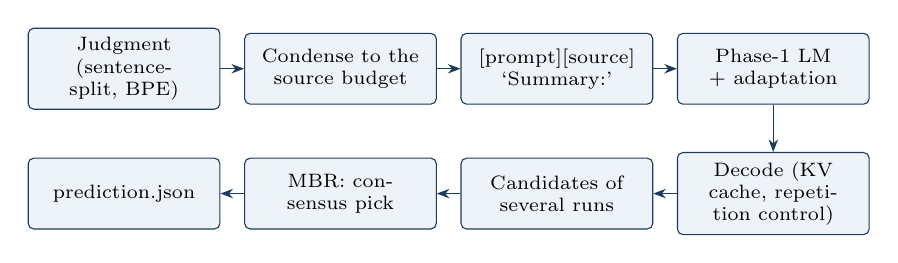
\begin{tikzpicture}[node distance=3mm, box/.style={draw=navy,rounded corners=2pt,fill=soft,align=center,
  font=\scriptsize,minimum height=9mm,text width=22mm}, arr/.style={-{Stealth[length=1.6mm]},navy}]
  \node[box] (a) {Judgment (sentence-split, BPE)};
  \node[box,right=of a] (b) {Condense to the source budget};
  \node[box,right=of b] (c) {[prompt][source] `Summary:'};
  \node[box,right=of c] (d) {Phase-1 LM + adaptation};
  \node[box,below=6mm of d] (e) {Decode (KV cache, repetition control)};
  \node[box,left=of e] (f) {Candidates of several runs};
  \node[box,left=of f] (g) {MBR: consensus pick};
  \node[box,left=of g] (h) {prediction.json};
  \foreach \x/\y in {a/b,b/c,c/d,d/e,e/f,f/g,g/h} \draw[arr] (\x)--(\y);
\end{tikzpicture}
\caption{Pipeline (\code{p6/summ/}, \code{train.py}, \code{mbr.py}).}
\label{fig:model}\end{figure}

\begin{itemize}
  \item \textbf{Layout (A1, A3, A4).}  One sequence: a short prompt, the condensed source (left-padded), the
  separator ``\code{ Summary:}'', then the summary and end-of-sequence.  The loss is computed on the summary
  tokens only (up to 768 tokens; the median reference is about 770 tokens).  A3 attends bidirectionally over the
  prompt and source (its prefix-LM design) and causally over the summary.
  \item \textbf{A2 (encoder--decoder)} uses fusion-in-decoder \cite{izacard2021fid}: the source is split into
  4 chunks of 1{,}024 tokens, each encoded separately, and the decoder attends to all of them.
  \item \textbf{Long sources.}  Judgments have a median of about 3{,}100 words, more than the 1{,}024-token
  Phase-1 context.  A1's learned position table is linearly interpolated to the needed length
  \cite{chen2023pi} (re-interpolated when a run starts from a shorter-source run, \code{init\_run}); A3 (ALiBi)
  and A4 (RoPE) extrapolate without changes.  Budgets: 1{,}280 tokens (first round), 2{,}560, 4{,}096, 6{,}144
  and 8{,}192 (later rounds).
  \item \textbf{Condensation} (\code{summ/data.py}) when a document exceeds the budget: \emph{salient}
  (default) keeps the opening of the case (15\% of the budget; 30\% in S7c) plus the sentences closest to the
  document's TF-IDF centroid, in document order; \emph{spread} (S2) keeps evenly spaced sentences.
  \item \textbf{Decoding}: greedy with a KV cache, 300--800 new tokens.  The first decode of the first round
  used no repetition penalty and blocked repeated 4-grams; all later decodes use repetition penalty 1.15
  \cite{keskar2019ctrl} and block repeated 3-grams.  Beam search (4 beams) and sampling ($T=0.7$) were also
  tried.
\end{itemize}

\subsection{Adaptation techniques}
\begin{itemize}
  \item \textbf{Full fine-tuning}: F1 (A4), F2 (A2), L2 (A1), L3 (A3) and all long-source runs S*.
  \item \textbf{LoRA} \cite{hu2022lora} (E2, S2; A1): $r=32$, $\alpha=64$.
  \item \textbf{LoRMA} \cite{bihany2025lorma} (E1; A4): $W=(I+\tfrac{\alpha}{r}BA)W_0$, $r=32$, $\alpha=64$.
  \item \textbf{QLoRA} \cite{dettmers2023qlora} (E4; A2 + FiD): frozen weights in 4-bit NF4, LoRA $r=32$.
  \item \textbf{AdaLoRA} \cite{zhang2023adalora} (E6; A1): SVD-form update, rank pruned from 32 to 16.
  \item \textbf{Houlsby adapters} \cite{houlsby2019adapters} (E3; A3): bottleneck 128.
  \item \textbf{Prefix tuning} \cite{li2021prefix} (E5; A3): 64 learned key/value positions per layer from a
  512-wide MLP, implemented as a pre-filled KV cache.
  \item \textbf{Prompt tuning} \cite{lester2021prompt} (E7; A4): 64 learned input embeddings.
  \item \textbf{Knowledge distillation} \cite{hinton2015kd} (K1): the student is A4 with 6 of its 10 blocks
  (0, 2, 4, 5, 8, 9; global-attention layers kept), fully fine-tuned with
  $0.5\,\mathrm{CE} + 0.5\,T^2\,\mathrm{KL}(p^T_\text{teacher}\,\|\,p^T_\text{student})$ per summary token, $T=2$;
  the teacher is F1 (full A4).
\end{itemize}

\subsection{Training}
AdamW, 16 sequences per optimizer step (micro-batches of 1--4 with gradient accumulation), linear warm-up
(100 steps; 50 for runs that continue another run) then cosine decay, weight decay 0.01, dropout 0.1, bf16.
First round: 4 epochs, learning rate $10^{-4}$ for full fine-tuning, $5\times10^{-4}$ for LoRA, LoRMA, QLoRA and
AdaLoRA, $10^{-3}$ for adapters and prefix tuning, $3\times10^{-3}$ for prompt tuning.  Later full fine-tuning
runs: 5--6 epochs, or 2--3 epochs at $4$--$5\times10^{-5}$ when continuing a shorter-source run (marked * in
\autoref{tab:results}: S4 from S3, S7 from S6, S8 from S7, S9 from S5, S3b from S1).  The state with the lowest
validation loss is kept; it then decodes the validation and test documents.

\subsection{Combining runs}
\begin{itemize}
  \item \textbf{Token-level ensemble} (\code{ensemble.py}): several models decode together, averaging their
  next-token log-probabilities.
  \item \textbf{Minimum-Bayes-risk (MBR) selection} \cite{kumar2004mbr} (\code{mbr.py}): for each document, every
  run's summary is a candidate; the candidate with the highest mean agreement (ROUGE-1 F1 + ROUGE-2 F1) with the
  other candidates is submitted.  No extra model is involved.
\end{itemize}

\subsection{Submissions}
\code{prediction.json} is a list of \code{\{"id", "summary"\}} for the \ntest{} test documents, at the root of
a zip.

% =====================================================================
\section{Results}
\subsection{All experiments}
\begin{table}[H]\centering
\caption{Validation results (\nval{} documents).  First round decoded with repetition control (``rp'').
Ep.\ = epochs (* continues a shorter-source run).  Loss = validation loss on summary tokens.}\label{tab:results}
\resizebox{\linewidth}{!}{\begin{tabular}{llllrrrrrrr}\toprule
Run & Arch & Method & Source & Ep. & Trainable & Loss & BERTScore F1 & ROUGE-1 & ROUGE-L & Words\\\midrule
\tabinput{tables/results.tex}
\bottomrule\end{tabular}}\end{table}

\begin{figure}[H]\centering
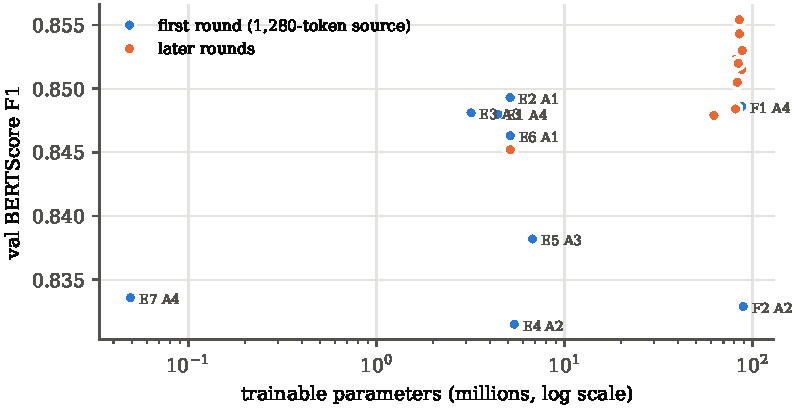
\includegraphics[width=0.85\linewidth]{figs/bs_vs_params.pdf}
\caption{Validation BERTScore F1 against the number of trained parameters.}
\label{fig:params}\end{figure}

\begin{figure}[H]\centering
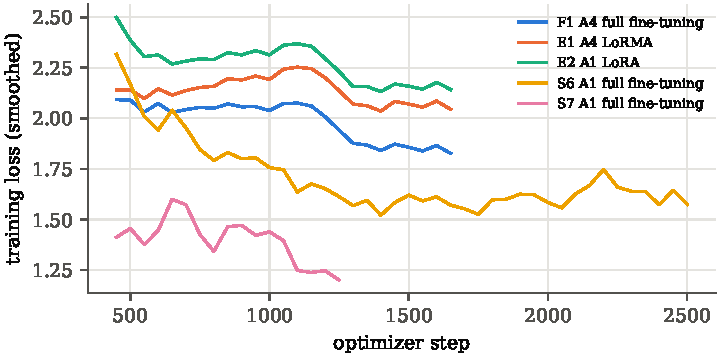
\includegraphics[width=0.8\linewidth]{figs/curves.pdf}
\caption{Training loss of selected runs (moving average).}
\label{fig:curves}\end{figure}

\subsection{Source length}
\begin{figure}[H]\centering
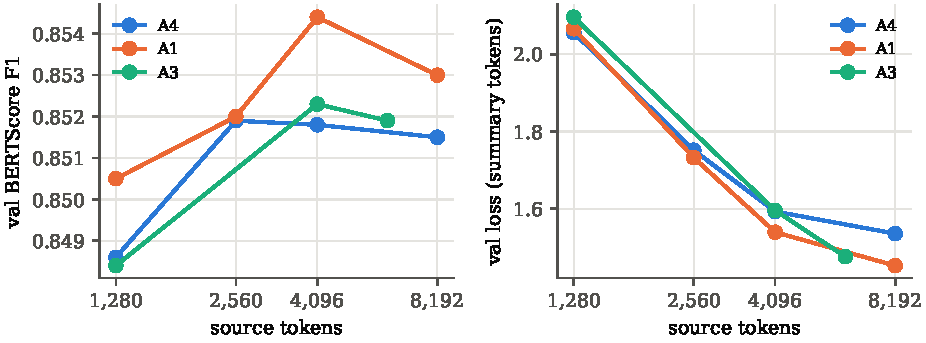
\includegraphics[width=0.95\linewidth]{figs/source_length.pdf}
\caption{Full fine-tuning with growing source budgets, per architecture (1{,}280-token points: F1, L2, L3).}
\label{fig:src}\end{figure}

\subsection{Decoding: repetition, length, beams, sampling}
\begin{table}[H]\centering\small
\caption{First-round runs, first decode (penalty 1.0, no repeated 4-grams) vs.\ repetition control
(penalty 1.15, no repeated 3-grams).  Distinct = share of distinct word trigrams per summary.}\label{tab:dec}
\resizebox{\linewidth}{!}{\begin{tabular}{lllrrrrrrrr}\toprule
& & & \multicolumn{2}{c}{BERTScore F1} & \multicolumn{2}{c}{ROUGE-1} & \multicolumn{2}{c}{Distinct 3-grams} & \multicolumn{2}{c}{Words}\\
Run & Arch & Method & first & rp & first & rp & first & rp & first & rp\\\midrule
\tabinput{tables/decoding.tex}
\bottomrule\end{tabular}}\end{table}

\begin{table}[H]\centering\small
\caption{Decoding variants: new-token range, repetition penalty, blocked n-gram size, search, number of
validation documents scored (not all variants were scored on all 300).}\label{tab:len}
\resizebox{\linewidth}{!}{\begin{tabular}{lllllrrrrrrr}\toprule
Run & New tokens & Pen. & No-rep. & Search & Docs & Words & BS-F1 & BS-P & BS-R & ROUGE-1 & ROUGE-L\\\midrule
\tabinput{tables/length.tex}
\bottomrule\end{tabular}}\end{table}

\subsection{Knowledge distillation and efficiency}
\begin{table}[H]\centering\small
\caption{Size, compute and memory.  Decode = seconds per validation document (batched).}\label{tab:eff}
\resizebox{\linewidth}{!}{\begin{tabular}{llllrrrrr}\toprule
Run & Arch & Method & Source & Total & Trainable & Train (min) & Decode (s/doc) & Peak GB\\\midrule
\tabinput{tables/efficiency.tex}
\bottomrule\end{tabular}}\end{table}
The KD student K1 has \kdparams{} parameters against \teacherparams{} for its teacher F1, and scores
\bsKone{} BERTScore F1 against \kdteacherrp{} for the teacher (same decoding).

\subsection{Combining runs}
\begin{table}[H]\centering\small
\caption{MBR selection and the token-level ensemble (validation).}\label{tab:mbr}
\begin{tabular}{lrrrrrr}\toprule
Name & Candidates & Docs & BERTScore F1 & ROUGE-1 & ROUGE-L & Words\\\midrule
\tabinput{tables/mbr.tex}
\bottomrule\end{tabular}\end{table}

\begin{table}[H]\centering\small
\caption{MBR7: share of validation documents for which each candidate run was picked (\%).}\label{tab:share}
\begin{tabular}{lr}\toprule Candidate & Picked (\%)\\\midrule
\tabinput{tables/mbr_share.tex}
\bottomrule\end{tabular}\end{table}

\subsection{Per-document scores}
\begin{figure}[H]\centering
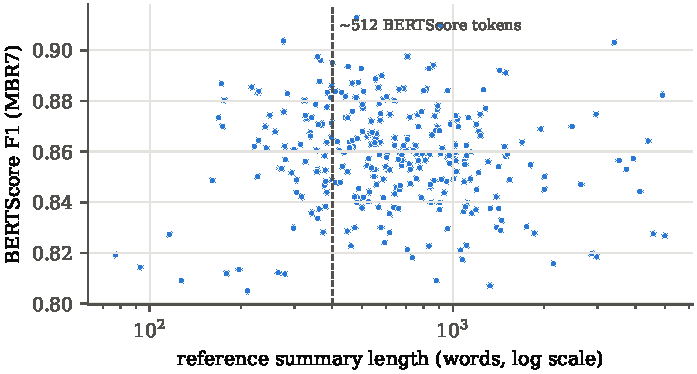
\includegraphics[width=0.75\linewidth]{figs/perdoc.pdf}
\caption{MBR7 BERTScore F1 per validation document against the reference length.  Correlation with reference
length \corrref; with log document length \corrdoc.}
\label{fig:perdoc}\end{figure}

\begin{table}[H]\centering\small
\caption{Mean BERTScore F1 by reference-length quartile (words).  MBR7 beats S7 on \mbrbetter\% of documents.}\label{tab:perdoc}
\begin{tabular}{llrrr}\toprule
Quartile & Reference words & Docs & MBR7 & S7\\\midrule
\tabinput{tables/perdoc.tex}
\bottomrule\end{tabular}\end{table}

\subsection{Submission files}
\nzips{} format-checked zips are in \code{p6/submissions/}.  Uploaded first: \code{MBR7\_all12} (\bsmbrseven,
ROUGE-1 \rougeonembrseven, ROUGE-L \rougelmbrseven), \code{MBR6\_long8} (\bsmbrsix), the best single models
S7 and S7c, and E1 (LoRMA) and K1 (KD) for technique coverage.
\authorbox{leaderboard scores}{Add the Codabench test BERTScore F1, ROUGE-1 and ROUGE-L of each uploaded submission
and say which six or more count towards the requirement.}
{\scriptsize\begin{longtable}{l}\toprule File\\\midrule\endhead
\tabinput{tables/submissions.tex}
\bottomrule\end{longtable}}

% =====================================================================
\section{Analysis}
\authorbox{analysis of the results}{The course rules do not allow LLM-written result analysis.  Questions the
course asks (§12.5), with the evidence above:
\begin{itemize}
  \item Which adaptation techniques are effective for legal summarization, and can parameter-efficient methods
  retain the quality of full adaptation (\autoref{tab:results}, \autoref{fig:params})?
  \item How do long-document strategies affect quality (condensation: E2 vs.\ S2; source length:
  \autoref{fig:src}; FiD for A2)?
  \item Do the summaries preserve important legal facts and reasoning?  (Read a sample of validation summaries
  next to their references.)
  \item How well do they cover important information (BERTScore recall, ROUGE)?
  \item How much redundancy and repetition is there (\autoref{tab:dec})?
  \item How does generation length affect BERTScore and ROUGE (\autoref{tab:len}, \autoref{tab:perdoc})?
  \item Does domain adaptation (Phase-1 pre-training on legal text) help?
  \item Does distillation preserve quality while reducing size and compute (\autoref{tab:eff})?
  \item How do model size, memory and inference cost change across experiments?
  \item Are the Phase-1 representations useful for abstractive summarization (compare with
  \autoref{tab:baselines})?
\end{itemize}}

\section{Limitations and next steps}
Facts that limit the conclusions (the interpretation is the author's):
\begin{itemize}
  \item The local BERTScore encoder (roberta-large) is probably not the organisers' ``legal BERTScore'', and it
  compares only about the first 400 words.
  \item Validation has \nval{} documents; differences of about 0.001 BERTScore are within noise.  One seed per
  run (S7b repeats S7 with another seed: \bsSsevenb{} vs.\ \bsSseven).
  \item The MBR candidate pool was chosen on the same validation split it is scored on.
  \item Some decoding variants were scored on 100 or 150 documents only (\autoref{tab:len}).
  \item The 1{,}024-token Phase-1 models were run at up to 8{,}192 tokens without long-context pre-training.
\end{itemize}
\authorbox{what you would do next}{With more time or compute: \ldots}

\section{Conclusions}
\authorbox{conclusions}{Summarise what you conclude from the experiments, in your own words.}

\section{Reproducibility}
\noindent{\small\begin{tabularx}{\linewidth}{l>{\raggedright\arraybackslash}X}
Token cache & built on first use by \code{summ/data.py} (\code{build\_cache})\\
Experiments & \code{bash run\_queue.sh f1\_a4\_full e1\_a4\_lorma ...} (one config each, logs in \code{logs/})\\
One experiment & \code{python train.py --config configs/s7\_a1\_full\_src4096.yaml}\\
Re-decode & \code{bash redecode.sh rp "gen.repetition\_penalty=1.15 gen.no\_repeat\_ngram=3" f1\_a4\_full ...}\\
MBR zip & \code{python mbr.py --name MBR7\_all12 --cand S7\_a1\_full\_src4096 S7\_a1\_full\_src4096:beam4 ...}\\
Token-level ensemble & \code{python ensemble.py --name ENS\_t3 --runs E2\_a1\_lora F1\_a4\_full E3\_a3\_adapter}\\
Figures and tables & \code{python p6/report/make\_figures.py}\\
\end{tabularx}}
\authorbox{repository link}{GitHub: \url{https://github.com/...}}

\section*{LLM declaration}
\authorbox{LLM declaration (mandatory)}{Fill in the course questionnaire.  Describe honestly which parts used
an LLM assistant (for example the data pipeline, model and training code, figures and this report's
methods/results text) and which parts are your own (design decisions, hyperparameters, analysis, conclusions).}

\begin{thebibliography}{99}\small
\bibitem{bihany2025lorma} H.~Bihany, S.~Patel, A.~Modi. LoRMA: Low-rank multiplicative adaptation for LLMs. Findings of ACL 2025.
\bibitem{chen2023pi} S.~Chen et al. Extending context window of large language models via positional interpolation. arXiv:2306.15595, 2023.
\bibitem{dettmers2023qlora} T.~Dettmers et al. QLoRA: Efficient finetuning of quantized LLMs. NeurIPS 2023.
\bibitem{hinton2015kd} G.~Hinton, O.~Vinyals, J.~Dean. Distilling the knowledge in a neural network. arXiv:1503.02531, 2015.
\bibitem{houlsby2019adapters} N.~Houlsby et al. Parameter-efficient transfer learning for NLP. ICML 2019.
\bibitem{hu2022lora} E.~J.~Hu et al. LoRA: Low-rank adaptation of large language models. ICLR 2022.
\bibitem{izacard2021fid} G.~Izacard, E.~Grave. Leveraging passage retrieval with generative models for open domain question answering. EACL 2021.
\bibitem{keskar2019ctrl} N.~S.~Keskar et al. CTRL: A conditional transformer language model for controllable generation. arXiv:1909.05858, 2019.
\bibitem{kumar2004mbr} S.~Kumar, W.~Byrne. Minimum Bayes-risk decoding for statistical machine translation. HLT-NAACL 2004.
\bibitem{lester2021prompt} B.~Lester, R.~Al-Rfou, N.~Constant. The power of scale for parameter-efficient prompt tuning. EMNLP 2021.
\bibitem{li2021prefix} X.~L.~Li, P.~Liang. Prefix-tuning: Optimizing continuous prompts for generation. ACL 2021.
\bibitem{zhang2023adalora} Q.~Zhang et al. AdaLoRA: Adaptive budget allocation for parameter-efficient fine-tuning. ICLR 2023.
\end{thebibliography}
\end{document}
